\begin{flushleft}
Abbiamo implementato il codice seguente per poter rispondere alle domande dell'esercizio:
\lstinputlisting[language=Matlab]{cap_3/es16/es16.m}
Possiamo confermare che le soluzioni $x$ e $y$ dei sistemi lineari $A\cdot x = b$ e $A\cdot y = c$ sono giuste dato che calcolando i loro residui otteniamo:
\begin{figure}[h]
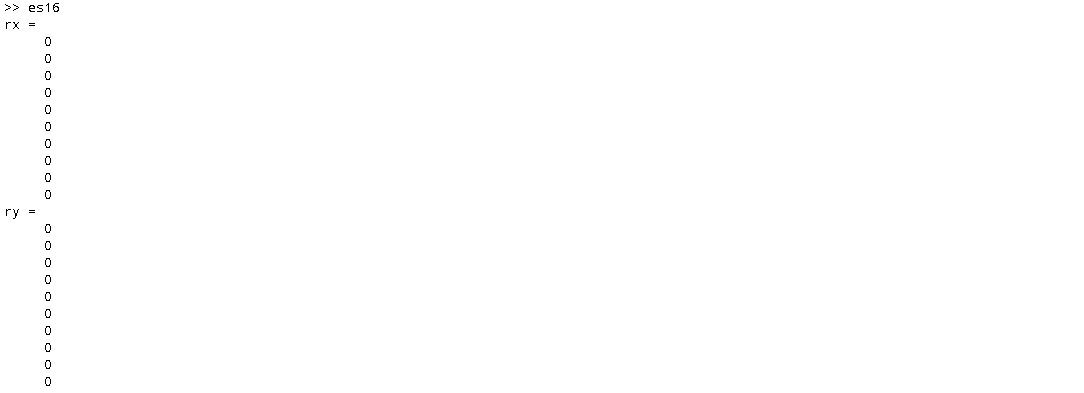
\includegraphics[left, width=250px]{cap_3/es16/es316}
\end{figure}
\newline \\
Nel passo successivo si usa la serie di istruzioni forniteci dall'esercizio. Nel caso del vettore $x$ si perviene alla stessa soluzione precedentemente fornita dall'esercizio. Invece nel caso del vettore $y$ abbiamo una propagazione degli errori nella soluzione trovata, che si può vedere a partire dall'elemento $y_7$. Possiamo vederlo dall'output:
\begin{figure}[h]
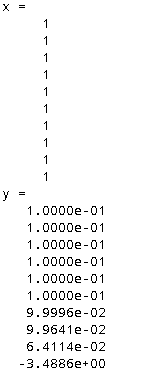
\includegraphics[left, width=250px]{cap_3/es16/es316a}
\end{figure}
\newline \\
Tuttavia questa propagazione degli errori non risulta essere malcondizionato come risulta della seguente differenza:
\begin{figure}[h]
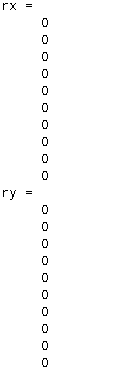
\includegraphics[left, width=250px]{cap_3/es16/es316b}
\end{figure}
\end{flushleft}